% Slides for 2024-01-17
% To create a slide, use the following:
% \begin{frame}{TITLE}
%     BODY
% \end{frame}

% To create a slide with a bullet list, use the following:
% \begin{frame}{TITLE}
%     \begin{itemize}
%         \item ITEM 1
%         \item ITEM 2
%     \end{itemize}    
% \end{frame}

% To create a slide with numbered list, use the following:
% \begin{frame}{TITLE}
%     \begin{enumerate}
%         \item ITEM 1
%         \item ITEM 2
%     \end{enumerate}
% \end{frame}

% To create a slide with a graphic:
% 1. Add the graphic to this folder (named picture.png)
% 2. Use the following:
% \begin{frame}{TITLE}
%     \centering
%     \includegraphics[height=0.7\textheight,width=0.7\textwidth,keepaspectratio]{picture.png}
% \end{frame}

% To create a slide with two columns, use the following:
% \begin{frame}{TITLE}
%     \begin{columns}
%         \begin{column}{0.5\textwidth}
%             COLUMN 1 BODY
%         \end{column}
%         \begin{column}{0.5\textwidth}
%             COLUMN 2 BODY
%         \end{column}
%     \end{columns}
% \end{frame}

\begin{frame}{Paper}
    \centering
    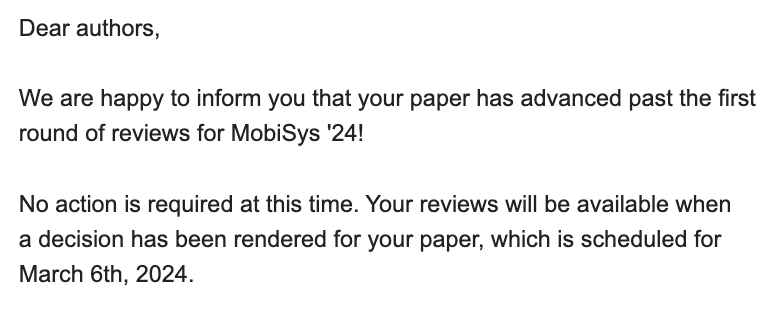
\includegraphics[height=0.7\textheight,width=0.7\textwidth,keepaspectratio]{fishsense_paper.png}
\end{frame}

\begin{frame}{Data Processing Results}
    Head/Tail stricter than necessary

    \begin{center}
    \begin{tabular}{ c | c | c | c }
        Topic & TP & TN & FP & FN\\
        \hline
        Overall & 12 & 43 & 37 & 18\\
        Laser & 78 & 16 & 9 & 7\\
        Head & 15 & 43 & 34 & 18\\
        Tail & 37 & 43 & 12 & 18
    \end{tabular}
    \end{center}
\end{frame}

\begin{frame}{Scalability}
    \begin{itemize}
        \item Run on AWS
        \item Label party
    \end{itemize}
\end{frame}

\tikzstyle{task} = [rectangle, rounded corners, 
minimum width=3cm, 
minimum height=1cm,
text centered, 
draw=black]
\tikzstyle{arrow} = [thick,->,>=stealth]
\begin{frame}
\frametitle{\textbf{Angle Estimation - Kunal and Avik}}
\begin{figure}
    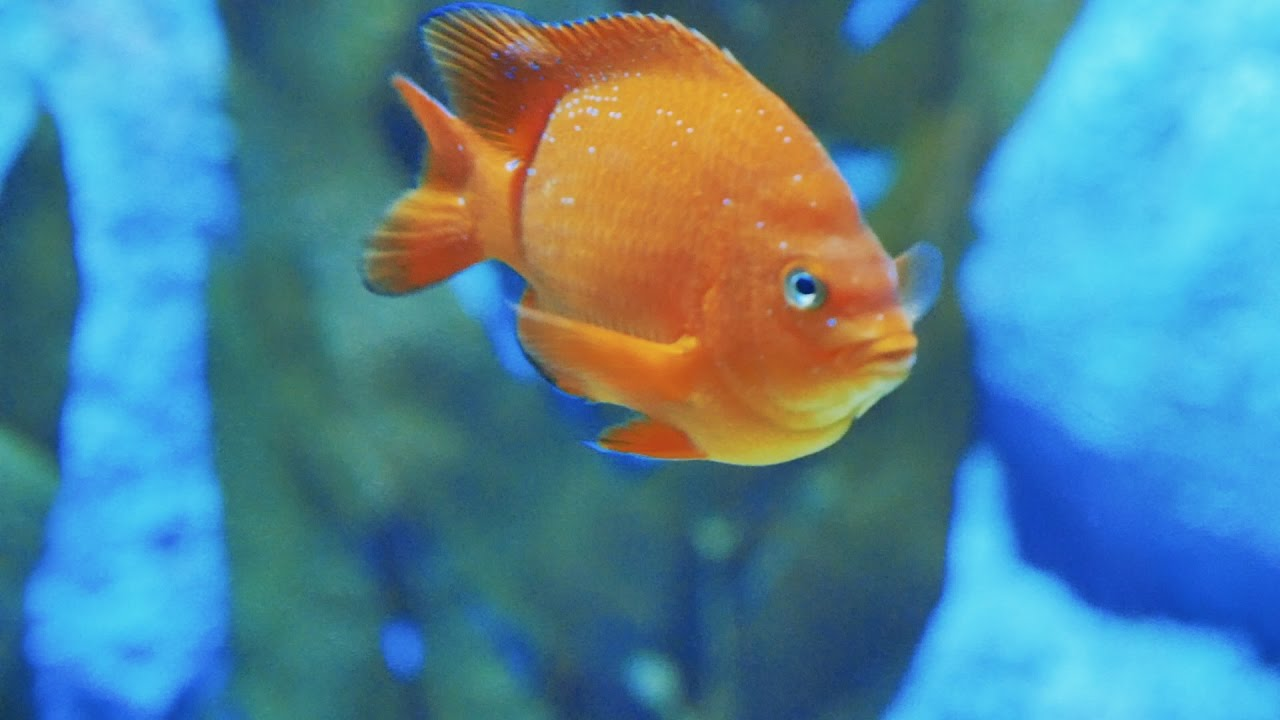
\includegraphics[width=0.5\linewidth]{fishswimming.png}
    \label{fig:fishswimming}
\end{figure}
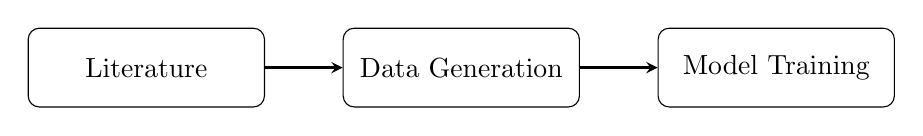
\begin{tikzpicture}[node distance=2cm]

\node (task1) [task] {Literature};
\node (task2) [task, right of=task1, xshift=2cm] {Data Generation};
\node (task3) [task, right of=task2, xshift=2cm] {Model Training};

\draw [arrow] (task1) -- (task2);
\draw [arrow] (task2) -- (task3);

\end{tikzpicture}
\end{frame}

\begin{frame}{Android/iOS App - CSE 145}
    \centering
    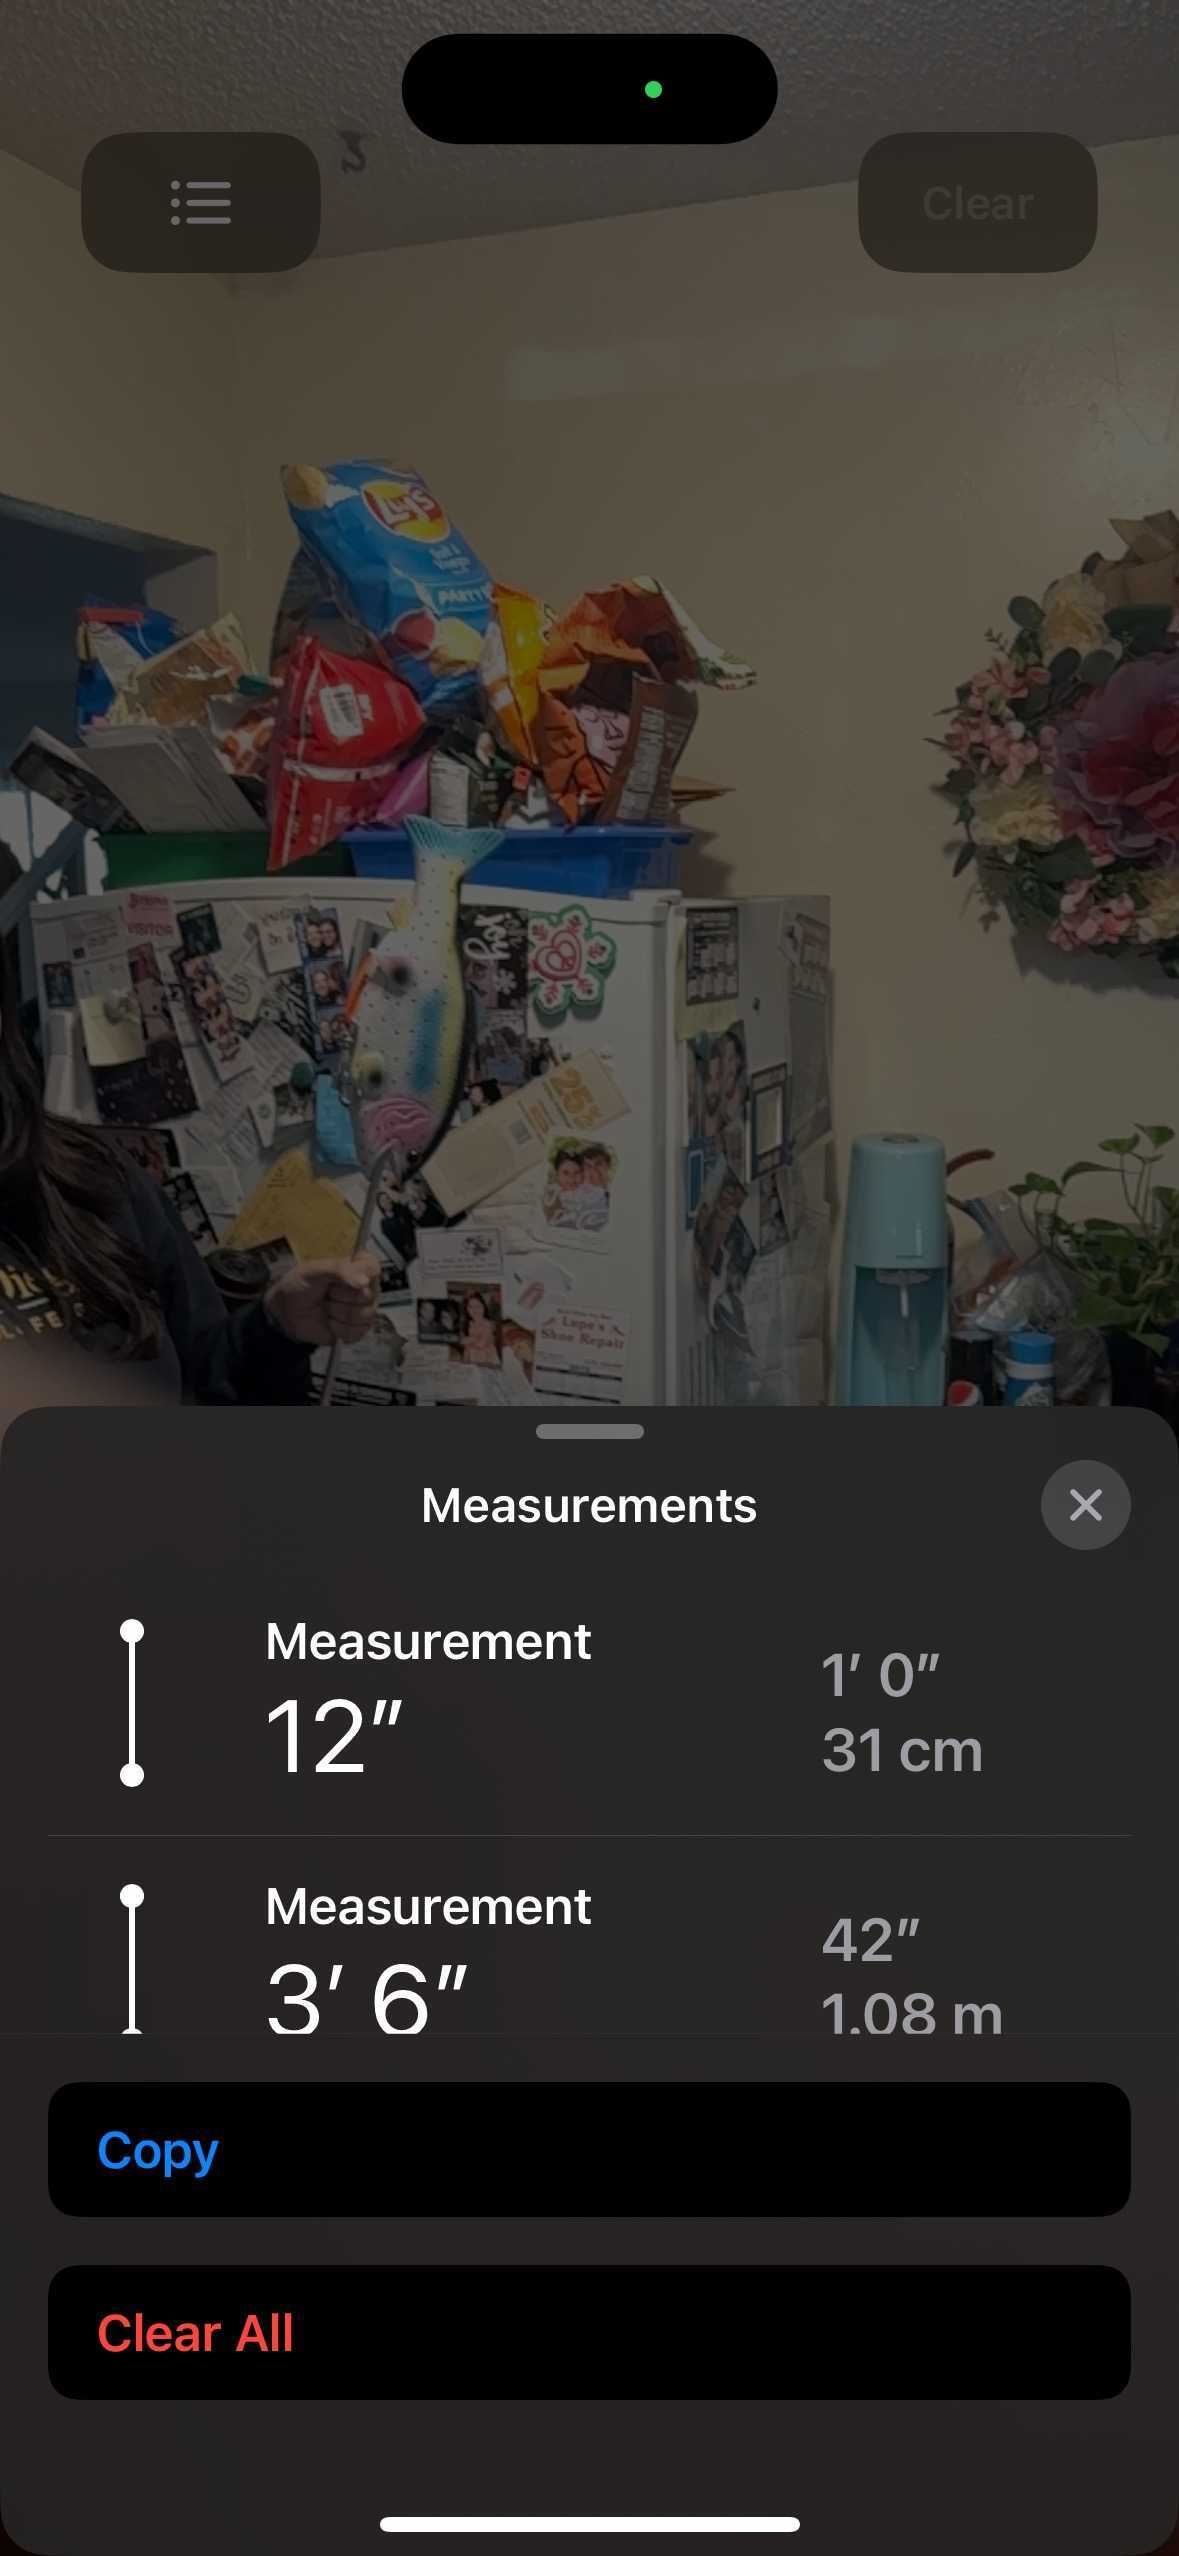
\includegraphics[height=0.7\textheight,width=0.7\textwidth,keepaspectratio]{fishsense_ios_measure.jpg}
\end{frame}
